\documentclass[11pt]{article}

% -------------------------------------------------------------------------------- %

% *** LANGUAGE ***
%\usepackage[italian]{babel}
%\usepackage[applemac]{inputenc}

% *** PAGE LAYOUT ***
\usepackage{geometry}     
%\geometry{a4paper}                   
%\geometry{landscape}                % Activate for for rotated page geometry
%\usepackage[parfill]{parskip}       % Activate to begin paragraphs with an empty line rather than an indent

\geometry{a4paper,tmargin=2cm,bmargin=2cm,lmargin=2.5cm,rmargin=2.5cm}

% *** DEFAULT FONT SELECTION ***
\usepackage[T1]{fontenc}
\usepackage{lmodern}
\renewcommand*\familydefault{\sfdefault} %	Only if the base font of the document is to be sans serif

% *** IMAGES ***
\usepackage{graphicx}
\usepackage{subfig}
\graphicspath{{C:/Users/Davide/Desktop/MAGISTRALE/1_ANNO/2_SEMESTRE/CONTROL_ENGENIREENG_LABORATORY/LAB1/MATLAB}}



\title{
	{\Large Laboratory report 2: Challenge \\
	 \large Group 2, Tuesday Shift}
}
\author{Baron Davide, Bonetto Alessio, Mustacchi Marco, Piron Luca Vittorio}
\date{April 26, 2022}


\begin{document}

\maketitle

\section{Introduction}

	\subsection{Activity Goal}
	The goal of the challenge of this laboratory is to design a control system for QUANSER SRV-02 MOTOR such that:

	\begin{itemize}
		\item It ensures asymptotic tracking of step references;
		\item It ensures an overshoot $M_p \le 10\%$ for a 60deg step reference;
		\item It attains a settling time $t_{s,5\%} \le 0.2s$ for the same reference;
		\item It employs the longest possible sampling time $T_S$.
	\end{itemize}

	\subsection{Model used}
	The black box $\textit{Quanser\_SRV02\_block}$ has been used in order to replace the DC motors physically present in the laboratory
	and faithfully reproduce the behaviour of the real one.


\section{Choice of control technique}

Among the possible solutions a control in state space has been chosen. 
The state space controller has been chosen instead of a PID controller because through a feedback it is possible to allocate more precisely the poles' location. \\
The direct design method has been choosen instead of emulation method because the first one is more robust with respect to the choiche of $T_S$.
Clearly, to ensures asymptotic tracking an integral control has been added in order to reduce the error modelling and the friction of the motor.



	\begin{figure}[h]
		\centering
		\subfloat[][]{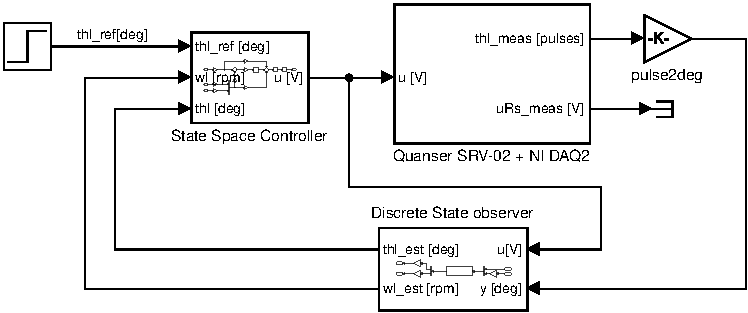
\includegraphics[scale=0.55]{images/System_model}}\quad
		\subfloat[][]{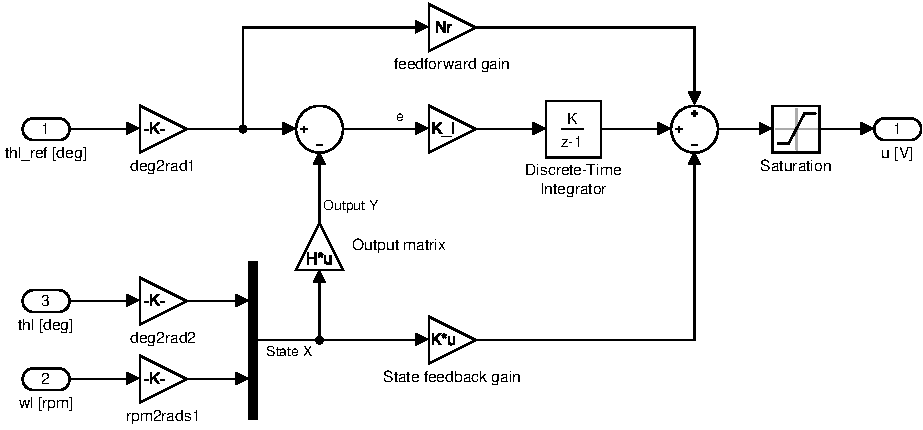
\includegraphics[scale=0.55]{images/Controller_model}}
		\caption{Simulink model used: full system with discrete-time observer (a); Discrete time controller with integrator and feedforward compensation (b).}
		\label{fig:model}
	\end{figure}
In the controller is also included a reduced order observer directly designed in discrete time as shown in Sec. 5.2 of the Handout, using the parameters evaluated in the next section.

\section{Choice of Parameters}
Through a trial-and-error approach the best sampling period $T_S$ has been obtained:
	\begin{equation}
		T_S=100\:ms
	\end{equation} 
Then, the following matrices has been used for the reduced order observer::
\begin{equation}
\Phi_o = 
	\left[
	\begin{array}{cccccc}
	1.3007\cdot 10^{-5} 
	\end{array}
	\right] ,
\qquad 
\Gamma_o 
= 
	\left[
	\begin{array}{ccc}
	4.6916  & -1.0100
	\end{array}
	\right]
\end{equation}

\begin{equation}
H_o
= 
	\left[
	\begin{array}{ccc}
	0 \\
	1
	\end{array}
	\right],
\qquad 
J_o
= 
	\left[
	\begin{array}{cc}
	0 & 1\\
	0 & L\\
	\end{array}
	\right]
\end{equation}
The feedback control gains, K and $K_I$, and the reduced observer gain L, are obtained by poles' location,as:
	\begin{equation}
		K = [4.6162 \:\:\:\:\:  0.0674] \quad K_I = 2.1307		\quad L = 1.01
	\end{equation} 
The feedforward gain has been obtained by trial-and-error:
	\begin{equation}
		N_r = 2.3
	\end{equation} 


\section{Results}
The best performances that the system is able to achieve with the chosen controller are:
	\begin{equation}
		 T_S = 100\:ms		\quad	t_{s,5\%} = 0.19999\:ms	\quad M_p =0.2\%
	\end{equation} 

	\begin{figure}[h!]
		\centering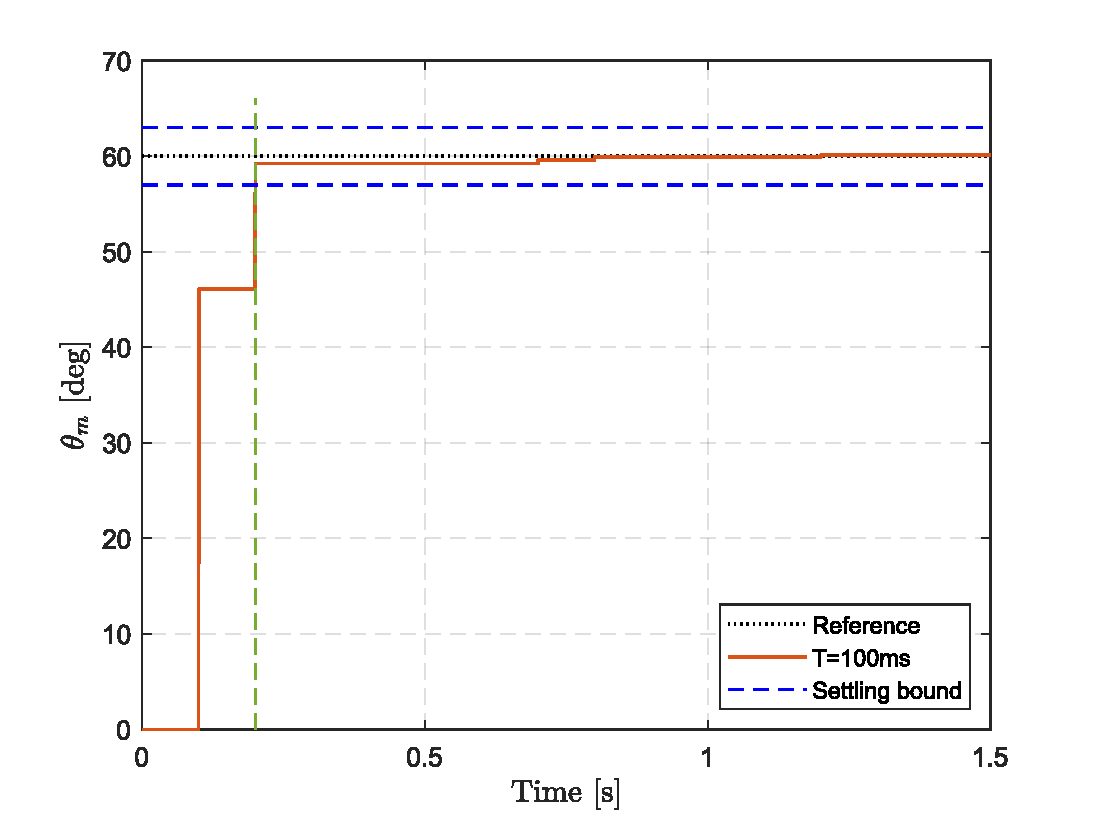
\includegraphics[scale=0.6]{images/Step_60}
		\caption{Step response to 60deg reference.}
	\end{figure}
			
\end{document}
